\documentclass[12pt,a4paper]{article}
\usepackage[utf8]{vietnam}
\usepackage{amsmath}
\usepackage{graphicx}
\usepackage{tikz}
\usepackage{algorithm}
\usepackage{algpseudocode}
\usepackage{geometry}
\usepackage{hyperref}
\usepackage{enumitem}
\usepackage{booktabs}

\geometry{margin=2.5cm}
\usetikzlibrary{shapes.geometric, arrows, positioning, fit, backgrounds}

\tikzstyle{process} = [rectangle, minimum width=3cm, minimum height=1cm, text centered, draw=black, fill=blue!20]
\tikzstyle{data} = [trapezium, trapezium left angle=70, trapezium right angle=110, minimum width=2cm, minimum height=1cm, text centered, draw=black, fill=green!20]
\tikzstyle{decision} = [diamond, minimum width=2cm, minimum height=1cm, text centered, draw=black, fill=yellow!20]
\tikzstyle{arrow} = [thick,->,>=stealth]
\tikzstyle{module} = [rectangle, rounded corners, minimum width=4cm, minimum height=1.5cm, text centered, draw=black, fill=orange!20, font=\bfseries]

\title{\textbf{Kiến Trúc Hệ Thống Tối Ưu Định Tuyến Phương Tiện \\ Sử Dụng Thuật Toán Di Truyền}}
\author{Hệ thống VRP-GA cho Logistics Việt Nam}
\date{\today}

\begin{document}

\maketitle
\tableofcontents
\newpage

\section{Tổng Quan Kiến Trúc Hệ Thống}

\subsection{Mô tả chung}
Hệ thống được thiết kế theo kiến trúc module hóa (modular architecture) với ba tầng chính:
\begin{itemize}
    \item \textbf{Tầng Dữ liệu (Data Layer)}: Xử lý và quản lý dữ liệu đầu vào
    \item \textbf{Tầng Tính toán (Computation Layer)}: Triển khai các thuật toán tối ưu
    \item \textbf{Tầng Trình bày (Presentation Layer)}: Trực quan hóa và đánh giá kết quả
\end{itemize}

\subsection{Sơ đồ kiến trúc tổng thể}

\begin{figure}[h]
\centering
\begin{tikzpicture}[node distance=2cm]

% Data Layer
\node (input) [data] {Dữ liệu đầu vào};
\node (preprocessing) [process, below of=input] {Tiền xử lý dữ liệu};
\node (distance) [process, below of=preprocessing] {Ma trận khoảng cách};

% Computation Layer
\node (vrp_model) [module, right of=preprocessing, xshift=4cm] {Mô hình VRP};
\node (ga_engine) [module, below of=vrp_model] {GA Engine};
\node (local_search) [module, below of=ga_engine] {Local Search (2-opt)};
\node (baseline) [module, right of=ga_engine, xshift=4cm] {Baseline Heuristic};

% Presentation Layer
\node (evaluation) [process, below of=local_search, yshift=-1cm] {Đánh giá KPI};
\node (visualization) [process, below of=evaluation] {Trực quan hóa};
\node (output) [data, below of=visualization] {Kết quả tối ưu};

% Arrows
\draw [arrow] (input) -- (preprocessing);
\draw [arrow] (preprocessing) -- (distance);
\draw [arrow] (distance) -- (vrp_model);
\draw [arrow] (vrp_model) -- (ga_engine);
\draw [arrow] (ga_engine) -- (local_search);
\draw [arrow] (preprocessing) -- (baseline);
\draw [arrow] (baseline) -- (evaluation);
\draw [arrow] (local_search) -- (evaluation);
\draw [arrow] (evaluation) -- (visualization);
\draw [arrow] (visualization) -- (output);

% Layer labels
\node[draw=red, thick, fit=(input) (preprocessing) (distance), inner sep=0.3cm, label=left:\textcolor{red}{\textbf{DATA LAYER}}] {};
\node[draw=blue, thick, fit=(vrp_model) (ga_engine) (local_search) (baseline), inner sep=0.3cm, label=right:\textcolor{blue}{\textbf{COMPUTATION LAYER}}] {};
\node[draw=green!50!black, thick, fit=(evaluation) (visualization) (output), inner sep=0.3cm, label=left:\textcolor{green!50!black}{\textbf{PRESENTATION LAYER}}] {};

\end{tikzpicture}
\caption{Kiến trúc tổng thể hệ thống VRP-GA}
\end{figure}

\newpage

\section{Kiến Trúc Chi Tiết Các Module}

\subsection{Module 1: Data Processing (Xử lý Dữ liệu)}

\subsubsection{Chức năng}
\begin{itemize}
    \item Thu thập và chuẩn hóa dữ liệu đầu vào
    \item Tạo ma trận khoảng cách giữa các điểm
    \item Xác định ràng buộc và tham số hệ thống
\end{itemize}

\subsubsection{Thành phần}

\begin{table}[h]
\centering
\begin{tabular}{@{}lll@{}}
\toprule
\textbf{Component} & \textbf{Chức năng} & \textbf{Output} \\ \midrule
Data Generator & Tạo dữ liệu mô phỏng & Tọa độ khách hàng \\
Demand Simulator & Mô phỏng nhu cầu & Demand vector \\
Distance Calculator & Tính khoảng cách & Distance matrix \\
Constraint Handler & Xử lý ràng buộc & Vehicle capacity \\ \bottomrule
\end{tabular}
\caption{Các thành phần của Data Processing Module}
\end{table}

\subsubsection{Cấu trúc dữ liệu}

\begin{algorithm}
\caption{Cấu trúc dữ liệu đầu vào}
\begin{algorithmic}[1]
\State \textbf{Input Data Structure:}
\State \hspace{0.5cm} $customers = \{c_1, c_2, ..., c_n\}$
\State \hspace{0.5cm} $coordinates = \{(x_i, y_i) | i = 1..n\}$
\State \hspace{0.5cm} $demands = \{d_i | i = 1..n, d_i \sim Poisson(\lambda)\}$
\State \hspace{0.5cm} $depot = \{x_0, y_0\}$
\State \hspace{0.5cm} $vehicles = \{v_1, v_2, ..., v_m\}$
\State \hspace{0.5cm} $capacity = Q$ (đơn vị hàng hóa/xe)
\State \hspace{0.5cm} $distance\_matrix[i][j] = euclidean(c_i, c_j) \times traffic\_factor$
\end{algorithmic}
\end{algorithm}

\subsection{Module 2: VRP Model (Mô hình bài toán)}

\subsubsection{Mô hình toán học}

Bài toán VRP được định nghĩa như sau:

\textbf{Biến quyết định:}
\begin{equation}
x_{ij}^k = \begin{cases}
1 & \text{nếu xe } k \text{ đi từ } i \text{ đến } j \\
0 & \text{ngược lại}
\end{cases}
\end{equation}

\textbf{Hàm mục tiêu:}
\begin{equation}
\min Z = \sum_{k=1}^{m} \sum_{i=0}^{n} \sum_{j=0}^{n} c_{ij} \cdot x_{ij}^k
\end{equation}

\textbf{Ràng buộc:}
\begin{align}
\sum_{k=1}^{m} \sum_{j=1}^{n} x_{ij}^k &= 1 \quad \forall i \in \{1,...,n\} \tag{Mỗi khách được phục vụ 1 lần}\\
\sum_{j=1}^{n} x_{0j}^k &= 1 \quad \forall k \tag{Mỗi xe xuất phát từ depot}\\
\sum_{i=1}^{n} x_{i0}^k &= 1 \quad \forall k \tag{Mỗi xe trở về depot}\\
\sum_{i \in S} d_i \cdot \sum_{j \notin S} x_{ij}^k &\leq Q \quad \forall k, S \subseteq \{1,...,n\} \tag{Ràng buộc sức chứa}
\end{align}

\subsection{Module 3: Genetic Algorithm Engine}

\subsubsection{Kiến trúc GA Engine}

\begin{figure}[h]
\centering
\begin{tikzpicture}[node distance=1.5cm]

\node (init) [process] {Khởi tạo quần thể};
\node (eval) [process, below of=init] {Đánh giá fitness};
\node (check) [decision, below of=eval, yshift=-0.5cm] {Đạt điều kiện \\ dừng?};
\node (selection) [process, below of=check, yshift=-1cm] {Selection};
\node (crossover) [process, below of=selection] {Crossover};
\node (mutation) [process, below of=crossover] {Mutation};
\node (output) [data, right of=check, xshift=4cm] {Best solution};

\draw [arrow] (init) -- (eval);
\draw [arrow] (eval) -- (check);
\draw [arrow] (check) -- node[anchor=west] {Không} (selection);
\draw [arrow] (selection) -- (crossover);
\draw [arrow] (crossover) -- (mutation);
\draw [arrow] (mutation) -- ++(3,0) |- (eval);
\draw [arrow] (check) -- node[anchor=south] {Có} (output);

\end{tikzpicture}
\caption{Workflow của GA Engine}
\end{figure}

\subsubsection{Thành phần chi tiết}

\textbf{1. Mã hóa nhiễm sắc thể (Chromosome Encoding):}

\begin{itemize}
    \item Mỗi cá thể = 1 chuỗi số nguyên đại diện cho thứ tự khách hàng
    \item Ví dụ: [3, 1, 5, 2, 4] nghĩa là xe đi: Depot $\rightarrow$ C3 $\rightarrow$ C1 $\rightarrow$ C5 $\rightarrow$ C2 $\rightarrow$ C4 $\rightarrow$ Depot
    \item Với nhiều xe: sử dụng delimiter hoặc split theo capacity
\end{itemize}

\textbf{2. Hàm fitness:}
\begin{equation}
fitness(individual) = \frac{1}{total\_distance(individual) + penalty}
\end{equation}

Trong đó:
\begin{itemize}
    \item $total\_distance$: tổng quãng đường của tất cả các tuyến
    \item $penalty$: phạt nếu vi phạm ràng buộc capacity
\end{itemize}

\textbf{3. Selection (Chọn lọc):}
\begin{itemize}
    \item Phương pháp: Tournament Selection
    \item Tournament size: 3-5 cá thể
    \item Elitism: giữ lại 10-20\% cá thể tốt nhất
\end{itemize}

\begin{algorithm}
\caption{Tournament Selection}
\begin{algorithmic}[1]
\Function{TournamentSelection}{$population, tournament\_size$}
    \State $tournament \gets$ random\_sample($population$, $tournament\_size$)
    \State $winner \gets$ individual with best fitness in $tournament$
    \State \Return $winner$
\EndFunction
\end{algorithmic}
\end{algorithm}

\textbf{4. Crossover (Lai ghép):}
\begin{itemize}
    \item Phương pháp: Order Crossover (OX) hoặc Partially Mapped Crossover (PMX)
    \item Xác suất crossover: $P_c = 0.8 - 0.9$
\end{itemize}

\begin{algorithm}
\caption{Order Crossover (OX)}
\begin{algorithmic}[1]
\Function{OrderCrossover}{$parent1, parent2$}
    \State Chọn ngẫu nhiên 2 điểm cắt $start, end$
    \State $child \gets$ sao chép đoạn $[start:end]$ từ $parent1$
    \State Điền các gen còn lại từ $parent2$ theo thứ tự, bỏ qua gen đã có
    \State \Return $child$
\EndFunction
\end{algorithmic}
\end{algorithm}

\textbf{5. Mutation (Đột biến):}
\begin{itemize}
    \item Phương pháp: Swap mutation, Inversion mutation
    \item Xác suất mutation: $P_m = 0.1 - 0.2$
\end{itemize}

\begin{algorithm}
\caption{Swap Mutation}
\begin{algorithmic}[1]
\Function{SwapMutation}{$individual$}
    \State Chọn ngẫu nhiên 2 vị trí $i, j$
    \State Hoán đổi gen tại vị trí $i$ và $j$
    \State \Return $individual$
\EndFunction
\end{algorithmic}
\end{algorithm}

\subsubsection{Tham số GA}

\begin{table}[h]
\centering
\begin{tabular}{@{}ll@{}}
\toprule
\textbf{Tham số} & \textbf{Giá trị} \\ \midrule
Population size & 100-200 \\
Number of generations & 500-1000 \\
Crossover probability & 0.8-0.9 \\
Mutation probability & 0.1-0.2 \\
Tournament size & 3-5 \\
Elitism rate & 10-20\% \\ \bottomrule
\end{tabular}
\caption{Tham số cấu hình GA}
\end{table}

\subsection{Module 4: Local Search (2-opt)}

\subsubsection{Mục đích}
Cải thiện nghiệm từ GA bằng cách loại bỏ các cạnh giao nhau trong lộ trình.

\subsubsection{Thuật toán 2-opt}

\begin{algorithm}
\caption{2-opt Local Search}
\begin{algorithmic}[1]
\Function{TwoOpt}{$route$}
    \State $improved \gets$ True
    \While{$improved$}
        \State $improved \gets$ False
        \For{$i \gets 0$ to $len(route) - 2$}
            \For{$j \gets i + 2$ to $len(route)$}
                \State $new\_route \gets$ Reverse($route[i+1:j]$)
                \If{Distance($new\_route$) $<$ Distance($route$)}
                    \State $route \gets new\_route$
                    \State $improved \gets$ True
                \EndIf
            \EndFor
        \EndFor
    \EndWhile
    \State \Return $route$
\EndFunction
\end{algorithmic}
\end{algorithm}

\subsubsection{Ví dụ minh họa}

Giả sử có lộ trình: A $\rightarrow$ B $\rightarrow$ C $\rightarrow$ D $\rightarrow$ E

\begin{itemize}
    \item Nếu cạnh AB và CD giao nhau
    \item 2-opt sẽ đảo ngược đoạn BC thành: A $\rightarrow$ C $\rightarrow$ B $\rightarrow$ D $\rightarrow$ E
    \item Kiểm tra xem có cải thiện khoảng cách không
\end{itemize}

\subsection{Module 5: Baseline Heuristic (Nearest Neighbor)}

\subsubsection{Mục đích}
Cung cấp nghiệm baseline để so sánh hiệu quả của GA.

\begin{algorithm}
\caption{Nearest Neighbor Heuristic}
\begin{algorithmic}[1]
\Function{NearestNeighbor}{$customers, depot, capacity$}
    \State $routes \gets []$
    \State $unvisited \gets customers$
    \While{$unvisited$ is not empty}
        \State $route \gets [depot]$
        \State $current \gets depot$
        \State $load \gets 0$
        \While{$unvisited$ is not empty}
            \State $nearest \gets$ argmin$_{c \in unvisited}$ distance($current, c$)
            \If{$load + demand[nearest] \leq capacity$}
                \State Add $nearest$ to $route$
                \State $load \gets load + demand[nearest]$
                \State Remove $nearest$ from $unvisited$
                \State $current \gets nearest$
            \Else
                \State \textbf{break}
            \EndIf
        \EndWhile
        \State Add $depot$ to $route$
        \State Append $route$ to $routes$
    \EndWhile
    \State \Return $routes$
\EndFunction
\end{algorithmic}
\end{algorithm}

\subsection{Module 6: Evaluation \& Visualization}

\subsubsection{KPI Metrics}

\begin{table}[h]
\centering
\begin{tabular}{@{}lll@{}}
\toprule
\textbf{KPI} & \textbf{Công thức} & \textbf{Đơn vị} \\ \midrule
Tổng quãng đường & $\sum_{k=1}^{m} distance(route_k)$ & km \\
Chi phí vận tải & $total\_distance \times cost\_per\_km$ & VNĐ \\
Số xe sử dụng & $m$ & xe \\
Tải trọng trung bình & $\frac{1}{m}\sum_{k=1}^{m} \frac{load_k}{Q} \times 100$ & \% \\
Thời gian tính toán & Runtime & giây \\ \bottomrule
\end{tabular}
\caption{Các chỉ số đánh giá hiệu suất}
\end{table}

\subsubsection{Visualization Components}

\begin{itemize}
    \item \textbf{Route Map}: Hiển thị lộ trình trên bản đồ Hà Nội (Folium)
    \item \textbf{Convergence Plot}: Biểu đồ fitness qua các thế hệ
    \item \textbf{Comparison Chart}: So sánh GA vs Baseline
    \item \textbf{Statistics Dashboard}: Bảng thống kê KPI
\end{itemize}

\newpage

\section{Workflow Tổng Thể}

\subsection{Quy trình xử lý end-to-end}

\begin{algorithm}
\caption{Main Workflow}
\begin{algorithmic}[1]
\State \textbf{Phase 1: Data Preparation}
\State $customers \gets$ GenerateCustomers($n=50$, area=HaNoi)
\State $demands \gets$ SimulateDemands(distribution=Poisson)
\State $distance\_matrix \gets$ CalculateDistances($customers$, traffic\_factor=$1.3$)

\State \textbf{Phase 2: Optimization}
\State $ga\_solution \gets$ GeneticAlgorithm($customers$, $vehicles$, $capacity$, $generations=1000$)
\State $ga\_solution \gets$ TwoOpt($ga\_solution$)
\State $nn\_solution \gets$ NearestNeighbor($customers$, $vehicles$, $capacity$)

\State \textbf{Phase 3: Evaluation}
\State $ga\_kpi \gets$ EvaluateKPI($ga\_solution$)
\State $nn\_kpi \gets$ EvaluateKPI($nn\_solution$)
\State $improvement \gets$ CompareResults($ga\_kpi$, $nn\_kpi$)

\State \textbf{Phase 4: Visualization}
\State PlotRoutes($ga\_solution$, map=HaNoi)
\State PlotConvergence($ga\_history$)
\State GenerateReport($ga\_kpi$, $nn\_kpi$, $improvement$)
\end{algorithmic}
\end{algorithm}

\subsection{Sơ đồ luồng dữ liệu}

\begin{figure}[h]
\centering
\begin{tikzpicture}[node distance=1.2cm, every node/.style={font=\small}]

\node (start) [data] {Dữ liệu thô};
\node (gen) [process, below of=start] {Tạo khách hàng};
\node (demand) [process, below of=gen] {Mô phỏng nhu cầu};
\node (dist) [process, below of=demand] {Tính khoảng cách};

\node (ga) [module, right of=dist, xshift=3cm] {GA Solver};
\node (opt) [process, below of=ga] {2-opt};
\node (nn) [module, right of=ga, xshift=3cm] {NN Solver};

\node (eval) [process, below of=opt, yshift=-0.5cm] {Đánh giá};
\node (compare) [process, below of=eval] {So sánh};
\node (viz) [process, below of=compare] {Trực quan};
\node (end) [data, below of=viz] {Báo cáo};

\draw [arrow] (start) -- (gen);
\draw [arrow] (gen) -- (demand);
\draw [arrow] (demand) -- (dist);
\draw [arrow] (dist) -- (ga);
\draw [arrow] (ga) -- (opt);
\draw [arrow] (dist) -- (nn);
\draw [arrow] (opt) -- (eval);
\draw [arrow] (nn) -- (eval);
\draw [arrow] (eval) -- (compare);
\draw [arrow] (compare) -- (viz);
\draw [arrow] (viz) -- (end);

\end{tikzpicture}
\caption{Data flow diagram}
\end{figure}

\newpage

\section{Triển Khai Kỹ Thuật}

\subsection{Stack công nghệ}

\begin{table}[h]
\centering
\begin{tabular}{@{}ll@{}}
\toprule
\textbf{Component} & \textbf{Technology} \\ \midrule
Programming Language & Python 3.8+ \\
GA Library & DEAP (Distributed EA in Python) \\
Optimization & OR-Tools (Google) \\
Data Processing & NumPy, Pandas \\
Visualization & Matplotlib, Folium \\
Geographic Data & OSRM API, Geopy \\
Testing & Pytest \\ \bottomrule
\end{tabular}
\caption{Stack công nghệ sử dụng}
\end{table}

\subsection{Cấu trúc thư mục dự án}

\begin{verbatim}
vrp-ga-system/
│
├── data/
│   ├── raw/                    # Dữ liệu gốc
│   ├── processed/              # Dữ liệu đã xử lý
│   └── benchmark/              # Solomon, CVRPLIB
│
├── src/
│   ├── data_processing/
│   │   ├── generator.py        # Tạo dữ liệu mô phỏng
│   │   ├── distance.py         # Tính khoảng cách
│   │   └── constraints.py      # Xử lý ràng buộc
│   │
│   ├── models/
│   │   ├── vrp_model.py        # Mô hình VRP
│   │   └── solution.py         # Cấu trúc nghiệm
│   │
│   ├── algorithms/
│   │   ├── genetic_algorithm.py    # GA engine
│   │   ├── operators.py            # Crossover, mutation
│   │   ├── local_search.py         # 2-opt
│   │   └── nearest_neighbor.py     # Baseline
│   │
│   ├── evaluation/
│   │   ├── metrics.py          # Tính KPI
│   │   └── comparator.py       # So sánh kết quả
│   │
│   └── visualization/
│       ├── mapper.py           # Vẽ bản đồ
│       ├── plotter.py          # Biểu đồ
│       └── reporter.py         # Tạo báo cáo
│
├── tests/                      # Unit tests
├── notebooks/                  # Jupyter notebooks
├── results/                    # Kết quả thực nghiệm
├── docs/                       # Tài liệu
└── main.py                     # Entry point
\end{verbatim}

\subsection{Ví dụ code chính}

\begin{verbatim}
# main.py
from src.data_processing import DataGenerator
from src.algorithms import GeneticAlgorithm, TwoOpt, NearestNeighbor
from src.evaluation import Evaluator
from src.visualization import RouteMapper

# 1. Data Preparation
generator = DataGenerator(n_customers=50, area="HaNoi")
customers = generator.generate_customers()
distance_matrix = generator.calculate_distances()

# 2. Solve with GA
ga = GeneticAlgorithm(
    population_size=100,
    generations=1000,
    crossover_prob=0.9,
    mutation_prob=0.15
)
ga_solution = ga.solve(customers, vehicles=5, capacity=100)
ga_solution = TwoOpt().improve(ga_solution)

# 3. Solve with baseline
nn_solution = NearestNeighbor().solve(customers, vehicles=5, capacity=100)

# 4. Evaluate
evaluator = Evaluator()
ga_kpi = evaluator.calculate_kpi(ga_solution)
nn_kpi = evaluator.calculate_kpi(nn_solution)

# 5. Visualize
mapper = RouteMapper()
mapper.plot_routes(ga_solution, title="GA Solution")
mapper.plot_comparison(ga_kpi, nn_kpi)
\end{verbatim}

\section{Kết Luận}

Kiến trúc hệ thống được thiết kế với các đặc điểm:
\begin{itemize}
    \item \textbf{Module hóa}: Dễ bảo trì và mở rộng
    \item \textbf{Linh hoạt}: Có thể thay đổi thuật toán, tham số
    \item \textbf{Scalable}: Xử lý được quy mô lớn hơn
    \item \textbf{Đánh giá toàn diện}: Nhiều KPI và phương pháp so sánh
    \item \textbf{Trực quan hóa tốt}: Giúp phân tích và báo cáo kết quả
\end{itemize}

Hệ thống có thể được mở rộng với:
\begin{itemize}
    \item Tích hợp dữ liệu thực tế từ doanh nghiệp logistics
    \item Thêm các ràng buộc: time windows, multiple depots, heterogeneous fleet
    \item Triển khai các thuật toán khác: ACO, PSO, Hybrid GA
    \item Xây dựng web interface hoặc API service
\end{itemize}

\newpage

\section{Phân Tích Chi Tiết Core Components}

\subsection{Core Component 1: GA Population Manager}

\subsubsection{Trách nhiệm}
Quản lý toàn bộ quần thể cá thể qua các thế hệ, bao gồm khởi tạo, lưu trữ, và cập nhật.

\subsubsection{Cấu trúc dữ liệu}

\begin{verbatim}
class Individual:
    chromosome: List[int]        # Chuỗi gene
    fitness: float               # Giá trị fitness
    routes: List[List[int]]      # Các tuyến đường
    total_distance: float        # Tổng quãng đường
    is_valid: bool              # Thỏa ràng buộc?
    
class Population:
    individuals: List[Individual]
    generation: int
    best_individual: Individual
    avg_fitness: float
    diversity: float            # Đa dạng quần thể
\end{verbatim}

\subsubsection{Các phương thức chính}

\begin{algorithm}
\caption{Population Initialization}
\begin{algorithmic}[1]
\Function{InitializePopulation}{$size, n\_customers, n\_vehicles$}
    \State $population \gets []$
    \For{$i \gets 1$ to $size$}
        \State $chromosome \gets$ RandomPermutation($1..n\_customers$)
        \State $routes \gets$ SplitIntoRoutes($chromosome, n\_vehicles$)
        \If{IsValid($routes$)}
            \State $individual \gets$ CreateIndividual($chromosome, routes$)
            \State Add $individual$ to $population$
        \Else
            \State Retry with penalty-based repair
        \EndIf
    \EndFor
    \State \Return $population$
\EndFunction
\end{algorithmic}
\end{algorithm}

\subsubsection{Chiến lược khởi tạo}

\begin{table}[h]
\centering
\begin{tabular}{@{}lll@{}}
\toprule
\textbf{Phương pháp} & \textbf{Mô tả} & \textbf{Tỷ lệ} \\ \midrule
Random & Hoán vị ngẫu nhiên & 60\% \\
Greedy & Dựa trên khoảng cách gần & 20\% \\
Cluster-first & Gom cụm trước, định tuyến sau & 15\% \\
Savings-based & Dựa trên Clarke-Wright & 5\% \\ \bottomrule
\end{tabular}
\caption{Chiến lược đa dạng hóa quần thể khởi tạo}
\end{table}

\subsection{Core Component 2: Fitness Evaluator}

\subsubsection{Hàm fitness đa mục tiêu}

\begin{equation}
Fitness = w_1 \cdot f_{distance} + w_2 \cdot f_{capacity} + w_3 \cdot f_{balance}
\end{equation}

Trong đó:
\begin{align}
f_{distance} &= \frac{1}{total\_distance + 1} \\
f_{capacity} &= penalty \times \sum_{k} \max(0, load_k - Q) \\
f_{balance} &= \frac{1}{\sigma(load_1, load_2, ..., load_m) + 1}
\end{align}

\subsubsection{Thuật toán đánh giá}

\begin{algorithm}
\caption{Fitness Evaluation}
\begin{algorithmic}[1]
\Function{EvaluateFitness}{$individual, distance\_matrix, capacity$}
    \State $routes \gets$ DecodeChromosome($individual.chromosome$)
    \State $total\_dist \gets 0$
    \State $penalty \gets 0$
    \State $loads \gets []$
    
    \For{each $route$ in $routes$}
        \State $route\_dist \gets$ CalculateRouteDistance($route, distance\_matrix$)
        \State $route\_load \gets \sum_{c \in route} demand[c]$
        \State $total\_dist \gets total\_dist + route\_dist$
        \State Add $route\_load$ to $loads$
        
        \If{$route\_load > capacity$}
            \State $penalty \gets penalty + 1000 \times (route\_load - capacity)$
        \EndIf
    \EndFor
    
    \State $balance\_factor \gets$ StandardDeviation($loads$)
    \State $fitness \gets \frac{1}{total\_dist + penalty + 10 \times balance\_factor}$
    \State \Return $fitness$
\EndFunction
\end{algorithmic}
\end{algorithm}

\subsection{Core Component 3: Crossover Operator}

\subsubsection{Các phương pháp crossover}

\textbf{1. Order Crossover (OX) - Chi tiết}

\begin{algorithm}
\caption{Order Crossover Implementation}
\begin{algorithmic}[1]
\Function{OrderCrossover}{$parent1, parent2$}
    \State $n \gets$ length($parent1$)
    \State $start \gets$ random($0, n-2$)
    \State $end \gets$ random($start+1, n-1$)
    
    \State $child \gets$ array of size $n$ filled with $-1$
    \State Copy $parent1[start:end]$ to $child[start:end]$
    
    \State $remaining \gets$ []
    \For{each gene $g$ in $parent2$}
        \If{$g$ not in $child$}
            \State Add $g$ to $remaining$
        \EndIf
    \EndFor
    
    \State $idx \gets end$
    \For{each gene $g$ in $remaining$}
        \State $child[idx \mod n] \gets g$
        \State $idx \gets idx + 1$
    \EndFor
    
    \State \Return $child$
\EndFunction
\end{algorithmic}
\end{algorithm}

\textbf{2. Partially Mapped Crossover (PMX)}

\begin{figure}[h]
\centering
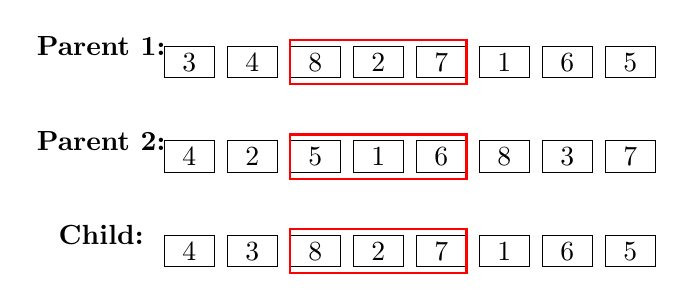
\begin{tikzpicture}[scale=0.8]
\node at (0,2) {\textbf{Parent 1:}};
\foreach \x/\val in {1/3, 2/4, 3/8, 4/2, 5/7, 6/1, 7/6, 8/5} {
    \draw (\x,1.5) rectangle (\x+0.8,2);
    \node at (\x+0.4,1.75) {\val};
}
\draw[red, thick] (3,1.4) rectangle (5.8,2.1);

\node at (0,0.5) {\textbf{Parent 2:}};
\foreach \x/\val in {1/4, 2/2, 3/5, 4/1, 5/6, 6/8, 7/3, 8/7} {
    \draw (\x,0) rectangle (\x+0.8,0.5);
    \node at (\x+0.4,0.25) {\val};
}
\draw[red, thick] (3,-0.1) rectangle (5.8,0.6);

\node at (0,-1) {\textbf{Child:}};
\foreach \x/\val in {1/4, 2/3, 3/8, 4/2, 5/7, 6/1, 7/6, 8/5} {
    \draw (\x,-1.5) rectangle (\x+0.8,-1);
    \node at (\x+0.4,-1.25) {\val};
}
\draw[red, thick] (3,-1.6) rectangle (5.8,-0.9);
\end{tikzpicture}
\caption{Ví dụ PMX Crossover}
\end{figure}

\textbf{3. Edge Recombination Crossover (ERX)}

Đặc biệt hiệu quả cho TSP-like problems:
\begin{itemize}
    \item Xây dựng edge map từ cả hai cha mẹ
    \item Chọn gene có ít neighbor nhất
    \item Giữ được cấu trúc edge tốt hơn
\end{itemize}

\subsection{Core Component 4: Mutation Operator}

\subsubsection{Các loại mutation}

\textbf{1. Swap Mutation}
\begin{verbatim}
Before: [1, 2, 3, 4, 5, 6, 7, 8]
               ↓        ↓
After:  [1, 2, 7, 4, 5, 6, 3, 8]
\end{verbatim}

\textbf{2. Inversion Mutation}
\begin{verbatim}
Before: [1, 2, 3, 4, 5, 6, 7, 8]
            └─────────┘
After:  [1, 2, 6, 5, 4, 3, 7, 8]
\end{verbatim}

\textbf{3. Insertion Mutation}
\begin{verbatim}
Before: [1, 2, 3, 4, 5, 6, 7, 8]
               ↓           ↑
After:  [1, 2, 4, 5, 6, 3, 7, 8]
\end{verbatim}

\textbf{4. Scramble Mutation}
\begin{verbatim}
Before: [1, 2, 3, 4, 5, 6, 7, 8]
            └─────────┘
After:  [1, 2, 5, 3, 6, 4, 7, 8] (random shuffle)
\end{verbatim}

\subsubsection{Adaptive Mutation Rate}

\begin{algorithm}
\caption{Adaptive Mutation}
\begin{algorithmic}[1]
\Function{AdaptiveMutation}{$individual, generation, max\_gen$}
    \State $base\_rate \gets 0.1$
    \State $progress \gets generation / max\_gen$
    
    \If{diversity is low}
        \State $mutation\_rate \gets base\_rate \times 2$
    \ElsIf{$progress > 0.8$}
        \State $mutation\_rate \gets base\_rate \times 0.5$ \Comment{Exploitation phase}
    \Else
        \State $mutation\_rate \gets base\_rate$
    \EndIf
    
    \If{random() $< mutation\_rate$}
        \State $mutation\_type \gets$ SelectMutationType($progress$)
        \State $individual \gets$ ApplyMutation($individual, mutation\_type$)
    \EndIf
    
    \State \Return $individual$
\EndFunction
\end{algorithmic}
\end{algorithm}

\subsection{Core Component 5: Route Decoder}

\subsubsection{Chuyển đổi chromosome thành routes}

\begin{algorithm}
\caption{Split Algorithm}
\begin{algorithmic}[1]
\Function{SplitIntoRoutes}{$chromosome, capacity, demands$}
    \State $routes \gets []$
    \State $current\_route \gets [depot]$
    \State $current\_load \gets 0$
    
    \For{each customer $c$ in $chromosome$}
        \If{$current\_load + demands[c] \leq capacity$}
            \State Add $c$ to $current\_route$
            \State $current\_load \gets current\_load + demands[c]$
        \Else
            \State Add $depot$ to $current\_route$
            \State Add $current\_route$ to $routes$
            \State $current\_route \gets [depot, c]$
            \State $current\_load \gets demands[c]$
        \EndIf
    \EndFor
    
    \State Add $depot$ to $current\_route$
    \State Add $current\_route$ to $routes$
    \State \Return $routes$
\EndFunction
\end{algorithmic}
\end{algorithm}

\subsubsection{Xử lý ràng buộc vi phạm}

\begin{algorithm}
\caption{Repair Mechanism}
\begin{algorithmic}[1]
\Function{RepairSolution}{$routes, capacity, demands$}
    \For{each $route$ in $routes$}
        \State $load \gets$ CalculateLoad($route, demands$)
        \While{$load > capacity$}
            \State $furthest \gets$ FindFurthestCustomer($route$)
            \State Remove $furthest$ from $route$
            \State Add $furthest$ to $unassigned\_customers$
            \State $load \gets load - demands[furthest]$
        \EndWhile
    \EndFor
    
    \For{each customer $c$ in $unassigned\_customers$}
        \State $best\_route \gets$ FindBestRoute($c, routes, capacity$)
        \State Insert $c$ into $best\_route$ at best position
    \EndFor
    
    \State \Return $routes$
\EndFunction
\end{algorithmic}
\end{algorithm}

\newpage

\section{Workflow Chi Tiết Từng Bước}

\subsection{Workflow 1: Data Preparation Pipeline}

\begin{figure}[h]
\centering
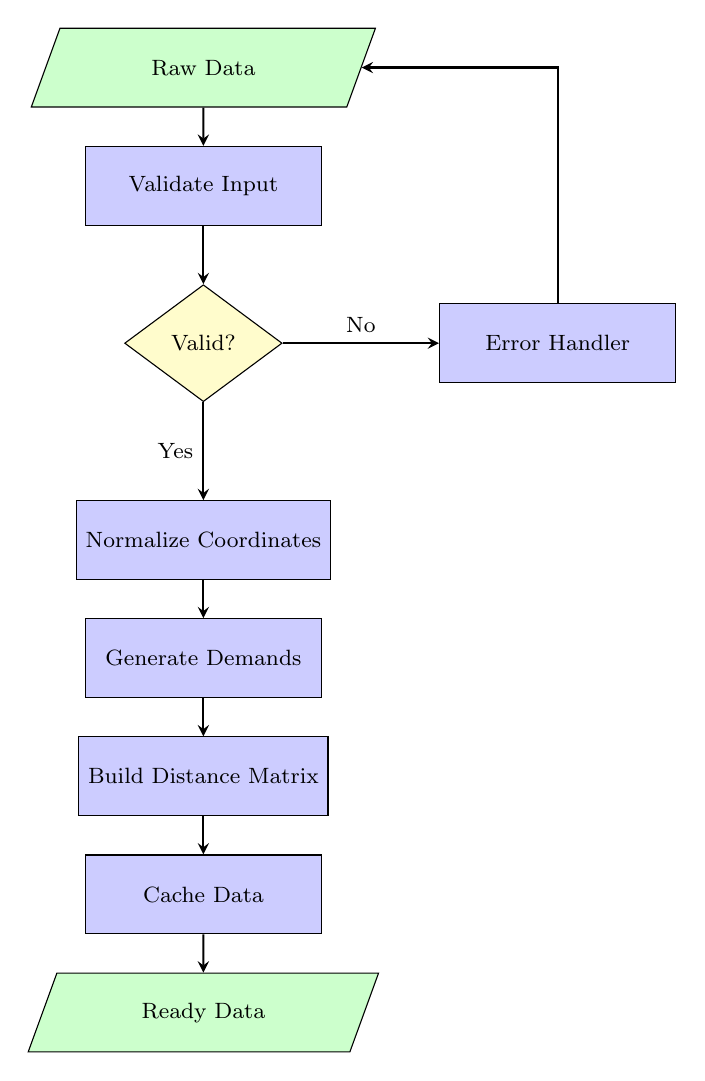
\begin{tikzpicture}[node distance=1.5cm, every node/.style={font=\footnotesize}]

\node (raw) [data] {Raw Data};
\node (validate) [process, below of=raw] {Validate Input};
\node (check1) [decision, below of=validate, yshift=-0.5cm] {Valid?};
\node (normalize) [process, below of=check1, yshift=-1cm] {Normalize Coordinates};
\node (demand) [process, below of=normalize] {Generate Demands};
\node (distance) [process, below of=demand] {Build Distance Matrix};
\node (cache) [process, below of=distance] {Cache Data};
\node (ready) [data, below of=cache] {Ready Data};

\node (error) [process, right of=check1, xshift=3cm] {Error Handler};

\draw [arrow] (raw) -- (validate);
\draw [arrow] (validate) -- (check1);
\draw [arrow] (check1) -- node[anchor=east] {Yes} (normalize);
\draw [arrow] (check1) -- node[anchor=south] {No} (error);
\draw [arrow] (normalize) -- (demand);
\draw [arrow] (demand) -- (distance);
\draw [arrow] (distance) -- (cache);
\draw [arrow] (cache) -- (ready);
\draw [arrow] (error) |- (raw);

\end{tikzpicture}
\caption{Data Preparation Workflow}
\end{figure}

\subsubsection{Chi tiết từng bước}

\textbf{Step 1: Validate Input}
\begin{itemize}
    \item Check số lượng khách hàng $> 0$
    \item Kiểm tra tọa độ hợp lệ
    \item Xác thực capacity $> 0$
    \item Đảm bảo số xe đủ để phục vụ
\end{itemize}

\textbf{Step 2: Normalize Coordinates}
\begin{equation}
x_{norm} = \frac{x - x_{min}}{x_{max} - x_{min}} \times scale
\end{equation}

\textbf{Step 3: Generate Demands}
\begin{itemize}
    \item Poisson distribution: $P(X=k) = \frac{\lambda^k e^{-\lambda}}{k!}$
    \item Typical $\lambda = 7$ (trung bình 7 đơn vị/khách)
    \item Clipping: $d_i \in [d_{min}, d_{max}]$
\end{itemize}

\textbf{Step 4: Build Distance Matrix}
\begin{equation}
d_{ij} = \sqrt{(x_i - x_j)^2 + (y_i - y_j)^2} \times traffic\_factor
\end{equation}

\subsection{Workflow 2: GA Execution Pipeline}

\begin{figure}[h]
\centering
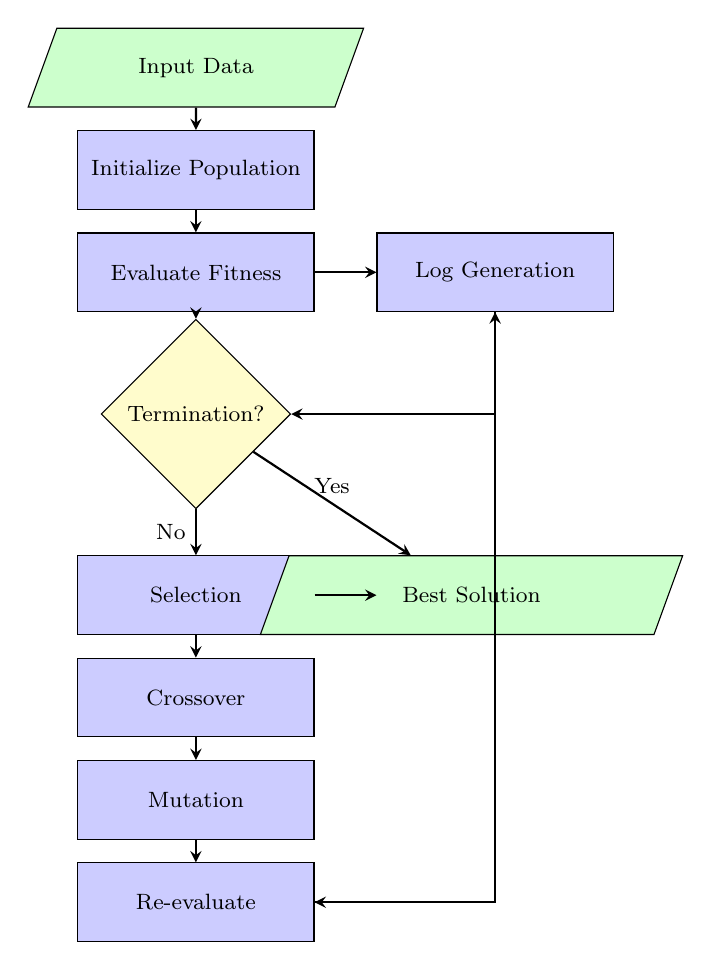
\begin{tikzpicture}[node distance=1.3cm, every node/.style={font=\footnotesize}]

\node (start) [data] {Input Data};
\node (init) [process, below of=start] {Initialize Population};
\node (eval1) [process, below of=init] {Evaluate Fitness};
\node (log1) [process, right of=eval1, xshift=2.5cm] {Log Generation};

\node (check) [decision, below of=eval1, yshift=-0.5cm] {Termination?};
\node (select) [process, below of=check, yshift=-1cm] {Selection};
\node (crossover) [process, below of=select] {Crossover};
\node (mutate) [process, below of=crossover] {Mutation};
\node (eval2) [process, below of=mutate] {Re-evaluate};
\node (elite) [process, right of=select, xshift=2.5cm] {Elitism};

\node (output) [data, below of=check, xshift=3.5cm, yshift=-1cm] {Best Solution};

\draw [arrow] (start) -- (init);
\draw [arrow] (init) -- (eval1);
\draw [arrow] (eval1) -- (check);
\draw [arrow] (eval1) -- (log1);
\draw [arrow] (check) -- node[anchor=east] {No} (select);
\draw [arrow] (check) -- node[anchor=south] {Yes} (output);
\draw [arrow] (select) -- (crossover);
\draw [arrow] (crossover) -- (mutate);
\draw [arrow] (mutate) -- (eval2);
\draw [arrow] (eval2) -| (log1);
\draw [arrow] (log1) |- (check);
\draw [arrow] (select) -- (elite);
\draw [arrow] (elite) |- (eval2);

\end{tikzpicture}
\caption{GA Execution Workflow}
\end{figure}

\subsubsection{Điều kiện dừng}

\begin{algorithm}
\caption{Termination Criteria}
\begin{algorithmic}[1]
\Function{CheckTermination}{$generation, best\_fitness, history$}
    \If{$generation \geq max\_generations$}
        \State \Return True
    \EndIf
    
    \If{$best\_fitness \geq target\_fitness$}
        \State \Return True
    \EndIf
    
    \State $recent \gets$ last 50 values in $history$
    \If{StandardDeviation($recent$) $< 0.001$}
        \State \Return True \Comment{Convergence}
    \EndIf
    
    \State \Return False
\EndFunction
\end{algorithmic}
\end{algorithm}

\subsection{Workflow 3: Local Search Optimization}

\begin{algorithm}
\caption{Complete 2-opt with Multi-route Support}
\begin{algorithmic}[1]
\Function{TwoOptAllRoutes}{$solution$}
    \State $improved \gets$ True
    \State $iteration \gets 0$
    
    \While{$improved$ and $iteration < max\_iterations$}
        \State $improved \gets$ False
        
        \For{each $route$ in $solution.routes$}
            \State $route \gets$ TwoOptSingleRoute($route$)
            \If{Distance($route$) improved}
                \State $improved \gets$ True
            \EndIf
        \EndFor
        
        \Comment{Inter-route optimization}
        \For{$i \gets 0$ to $len(routes)-2$}
            \For{$j \gets i+1$ to $len(routes)-1$}
                \State Try swapping customers between $route_i$ and $route_j$
                \If{Total distance improved}
                    \State Apply swap
                    \State $improved \gets$ True
                \EndIf
            \EndFor
        \EndFor
        
        \State $iteration \gets iteration + 1$
    \EndWhile
    
    \State \Return $solution$
\EndFunction
\end{algorithmic}
\end{algorithm}

\subsection{Workflow 4: Result Analysis Pipeline}

\begin{figure}[h]
\centering
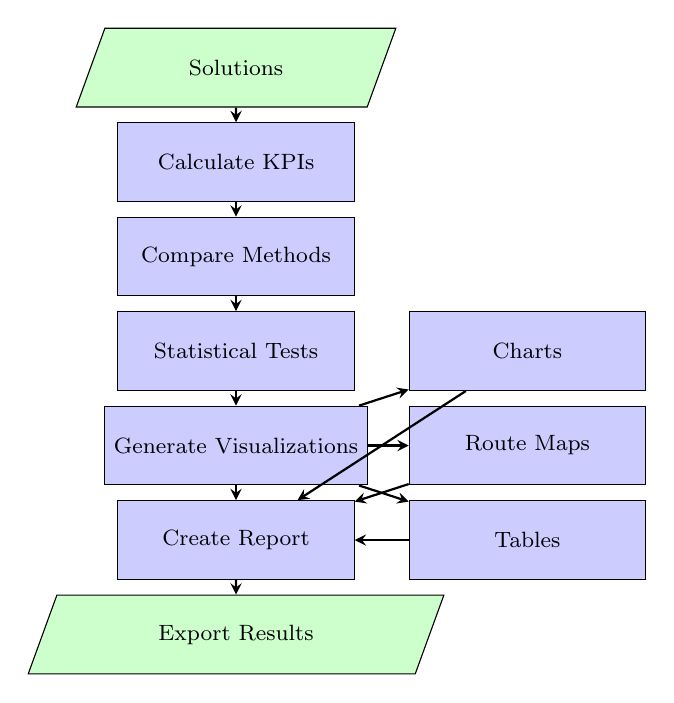
\begin{tikzpicture}[node distance=1.2cm, every node/.style={font=\footnotesize}]

\node (sol) [data] {Solutions};
\node (kpi) [process, below of=sol] {Calculate KPIs};
\node (compare) [process, below of=kpi] {Compare Methods};
\node (stat) [process, below of=compare] {Statistical Tests};
\node (viz) [process, below of=stat] {Generate Visualizations};
\node (report) [process, below of=viz] {Create Report};
\node (export) [data, below of=report] {Export Results};

\node (map) [process, right of=viz, xshift=2.5cm] {Route Maps};
\node (chart) [process, above of=map] {Charts};
\node (table) [process, below of=map] {Tables};

\draw [arrow] (sol) -- (kpi);
\draw [arrow] (kpi) -- (compare);
\draw [arrow] (compare) -- (stat);
\draw [arrow] (stat) -- (viz);
\draw [arrow] (viz) -- (report);
\draw [arrow] (report) -- (export);

\draw [arrow] (viz) -- (map);
\draw [arrow] (viz) -- (chart);
\draw [arrow] (viz) -- (table);
\draw [arrow] (map) -- (report);
\draw [arrow] (chart) -- (report);
\draw [arrow] (table) -- (report);

\end{tikzpicture}
\caption{Result Analysis Workflow}
\end{figure}

\newpage

\section{Tối Ưu Hiệu Năng}

\subsection{Parallel Processing}

\subsubsection{Fitness Evaluation Song Song}

\begin{verbatim}
from multiprocessing import Pool

def evaluate_population_parallel(population, n_workers=4):
    with Pool(processes=n_workers) as pool:
        fitness_values = pool.map(evaluate_fitness, population)
    
    for individual, fitness in zip(population, fitness_values):
        individual.fitness = fitness
    
    return population
\end{verbatim}

\subsubsection{Island Model GA}

\begin{figure}[h]
\centering
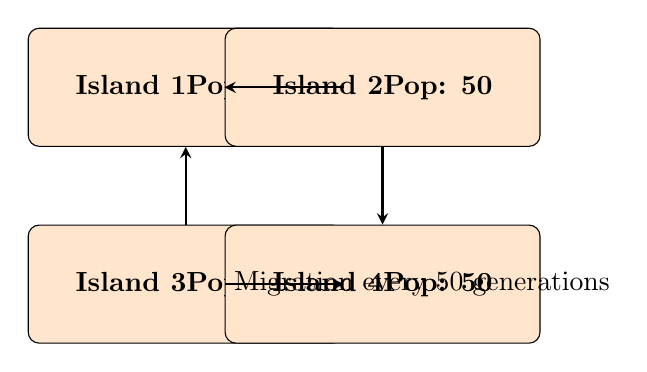
\begin{tikzpicture}[node distance=2.5cm]

\node (island1) [module] {Island 1\\Pop: 50};
\node (island2) [module, right of=island1] {Island 2\\Pop: 50};
\node (island3) [module, below of=island1] {Island 3\\Pop: 50};
\node (island4) [module, right of=island3] {Island 4\\Pop: 50};

\draw [arrow, bend left=20] (island1) -- (island2);
\draw [arrow, bend left=20] (island2) -- (island4);
\draw [arrow, bend left=20] (island4) -- (island3);
\draw [arrow, bend left=20] (island3) -- (island1);

\node at (3,-2.5) {Migration every 50 generations};

\end{tikzpicture}
\caption{Island Model for Parallel GA}
\end{figure}

\subsection{Caching Strategy}

\begin{table}[h]
\centering
\begin{tabular}{@{}lll@{}}
\toprule
\textbf{Cache Type} & \textbf{Data} & \textbf{Benefit} \\ \midrule
Distance Cache & $d_{ij}$ values & Avoid recalculation \\
Fitness Cache & Evaluated solutions & Skip duplicates \\
Route Cache & Valid route segments & Speed up decoding \\
2-opt Cache & Improved routes & Avoid redundant checks \\ \bottomrule
\end{tabular}
\caption{Caching mechanisms}
\end{table}

\subsection{Memory Optimization}

\begin{itemize}
    \item \textbf{Sparse Matrix}: Chỉ lưu khoảng cách $< threshold$
    \item \textbf{Integer Encoding}: Dùng int16 thay vì float64 cho gene
    \item \textbf{Lazy Evaluation}: Chỉ tính fitness khi cần
    \item \textbf{Generational GC}: Thu gom bộ nhớ sau mỗi thế hệ
\end{itemize}

\section{Error Handling \& Monitoring}

\subsection{Exception Handling}

\begin{verbatim}
class VRPException(Exception):
    pass

class InfeasibleSolutionError(VRPException):
    """No valid solution exists"""
    pass

class CapacityViolationError(VRPException):
    """Route exceeds vehicle capacity"""
    pass

def safe_ga_execution(data, params):
    try:
        solution = run_ga(data, params)
        return solution
    except InfeasibleSolutionError as e:
        logger.error(f"Infeasible problem: {e}")
        return None
    except CapacityViolationError as e:
        logger.warning(f"Capacity violation, applying repair: {e}")
        return repair_and_retry(data, params)
    except Exception as e:
        logger.critical(f"Unexpected error: {e}")
        raise
\end{verbatim}

\subsection{Monitoring Metrics}

\begin{table}[h]
\centering
\begin{tabular}{@{}ll@{}}
\toprule
\textbf{Metric} & \textbf{Purpose} \\ \midrule
Best fitness per generation & Track convergence \\
Average fitness & Monitor population quality \\
Diversity index & Prevent premature convergence \\
Constraint violations & Track feasibility \\
Execution time & Performance monitoring \\
Memory usage & Resource management \\ \bottomrule
\end{tabular}
\caption{Real-time monitoring metrics}
\end{table}

\end{document}